\documentclass[fleqn,10pt]{olplainarticle}
% Use option lineno for line numbers 

\title{Clinical Management of Pneumocephalus}

\author{Jocelyn Cheng}
\affil{MS3, Warren Alpert Medical School of Brown University}

\keywords{intracranial surgery, Mount Fuji sign, neurocritical care, tension pneumocephalus}

\begin{abstract}
Pneumocephalus (PNC) is when air enters the intracranial cavity. PNC is caused most frequently by trauma, infection or surgery. PNC causes neurodegeneration through free radical damage and mass effect; the characteristic "Mount Fuji sign" is caused by compression of frontal lobes with interhemispheric widening. We present our own case, in addition to the most relevant clinical features, diagnostic methods, and current management for this condition.
\end{abstract}

\begin{document}

\flushbottom
\maketitle
\thispagestyle{empty}

\section*{Introduction}

Pneumocephalus (\textit{"pneumo" = air} and \textit{cepahalus = head}) is the presence of air in the intracranial cavity. Air most frequently enters the subdural space, but may also occupy the epidural, subarachnoid, intraventricular, intracerebral space. Air most commonly collects in the frontal, followed by the occipital and temporal areas \citep{pmid23607059}.

\section*{Clinical Features of Pneumocephalus}
\label{sec:examples}
Pneumocephalus may cause headache, nausea, vomiting, irritability, dizziness, seizures or a “gurgling” sensation in the head  \citep{pmid15953284}. Tension pneumocephalous is a severe form of PNC that causes intracranial hypertension and mass effect, and can be fatal. \cite{pmid3335913} described the characteristic dual-peaked frontal lobes produced by interhemispheric collection of air as the Mt. Fuji sign (Figure~\ref{fig:Fuji}). 

\subsection*{Mechanism and Etiologies}
75\% of PNC cases are caused by trauma, 9\% are caused by infection (usually otitis media); other common causes of PNC include cranial, spinal, or ENT surgery \citep{pmid6032371}. 
\\
Three current hypotheses exist regarding the mechanism of PNC \citep{pmid26500801}: 
\\1. The ball valve effect. CSF leak following trauma allows inflow but not outflow of air. As incranial pressure rises, the brain and dura plug the fistula tract and prevent air from escaping, causing PNC.
\\2. The inverted soda bottle effect. Drainage of CSF causes a negative intracranial pressure differential. Air enters as bubbles through the CSF to equalize the pressure gradient.
\\3. Less commonly, gas producing organisms may form gas \textit{in situ}.


\subsection*{Diagnosis}
CT is the gold standard of PNC diagnosis. It is more sensitive than MRI for detecting intracranial air and requires only .55mL of air to detect PNC as compared the 2mL of air needed to detect PNC on plain radiograph \citep{pmid24305016}. The Mt. Fuji sign is generally an indicator of more severe PNC and can be useful in discriminating tension PNC from nontension PNC \citep{pmid15286317}. However, there are some cases of patients with Mt. Fuji signs that are managed nonoperatively and cases of patients with massive PNC that are asymptomatic \citep{pmid7142505}.

\subsection*{Treatment}
85\% of PNC cases resolve with conservative treatment \citep{pmid24305016}. Conservative treatment may involve placing the patient in a Fowler 30 degree incline, avoiding Valsalva/cough, hyperthermia prevention, and osmotic diuretics. However, other interventions, such as oxygen therapy and surgery may improve outcomes and air reabsorption time. \cite{pmid25992622} found that treatment with 3 hours of 100\% oxygen delivered via nasogastric tube was effective in increasing air resorption, alertness (measured via Stanford sleepyness test), decreased pneumocephalus volume, and had no change in attention (measured via Stroop test). Outcomes were most significantly improved in men, and patients with age >52 \citep{pmid25992622}. \cite{pmid25328392} demonstrated increased reabsorption of nitrogen and decreased volume of intracranial air in 13 patients with PNC treated with hyperbaric oxygen as compared to 11 normobaric controls treated continuously with 5L/min of oxygen. Hyperbaric patients were also found to have lower rates of meningitis and had shorter hospital stays. However, González Tortosa (1996) reported a case of PNC aggravated by hyperbaric oxygen therapy. \cite{pmid16379134} recommended 100\% oxygen therapy following bony dural defect. \cite{pmid18447708} found oxygen mask therapy to be more effective than nasal catheter in normobaric oxygen therapy. Symptomatic TP requires emergent surgical decompression to prevent permanent neurological deficit.

In summary, PNC  must be treated by surgical revision when it causes intracranial hypertension and/or deterioration of consciousness. Mt Fuji signs are often correlated with worse PNC. However, there are a few cases of patients with Mount Fuji signs that do not require surgical procedures. The conservative treatment in these patients may include Fowler incline, intracranial pressure control, hyperthermia prevention, and osmotic diuretics. Hyperbaric HBO2 therapy or normobaric oxygenation administered continuously at 5 L/min at least for 5 days may lead to clinical and radiological improvement as well as a reduction in hospitalization time.

\begin{figure}[ht]
\centering
\includegraphics[width=0.3\linewidth]{Fuji}
\caption{Mt. Fuji, Japan}
\label{fig:Fuji}
\end{figure}

\begin{figure}[ht]
\centering
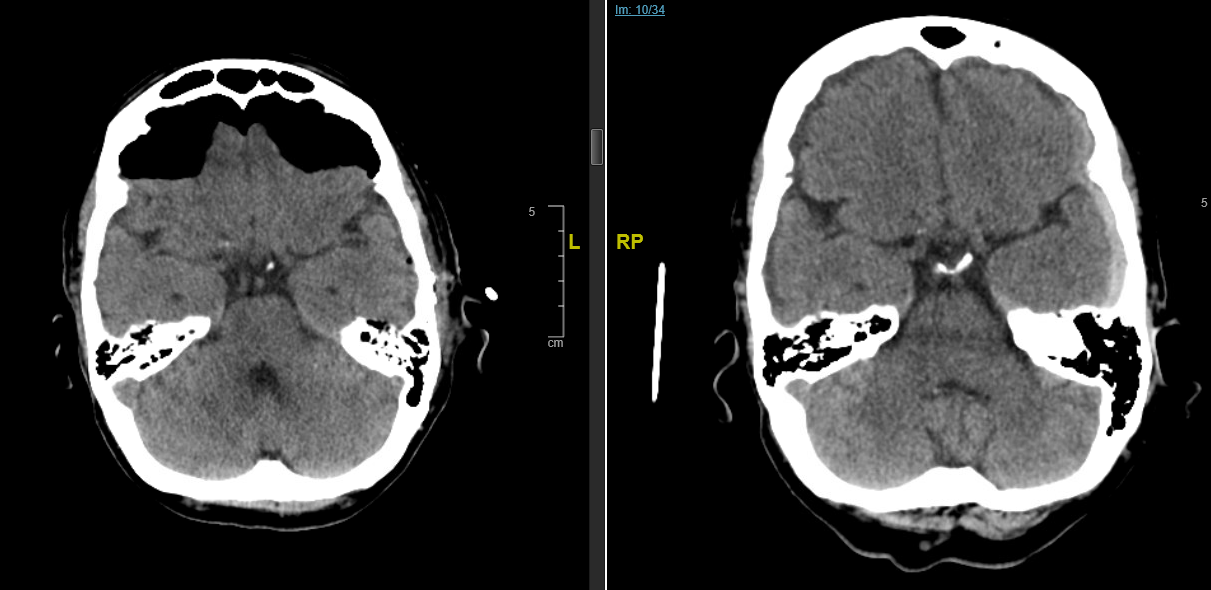
\includegraphics[width=0.7\linewidth]{CT}
\caption{CT Brain without contrast before (right) and after (left) craniotomy with characteristic Mt. Fuji sign}
\label{fig:view}
\end{figure}

\begin{figure}[ht]
\centering
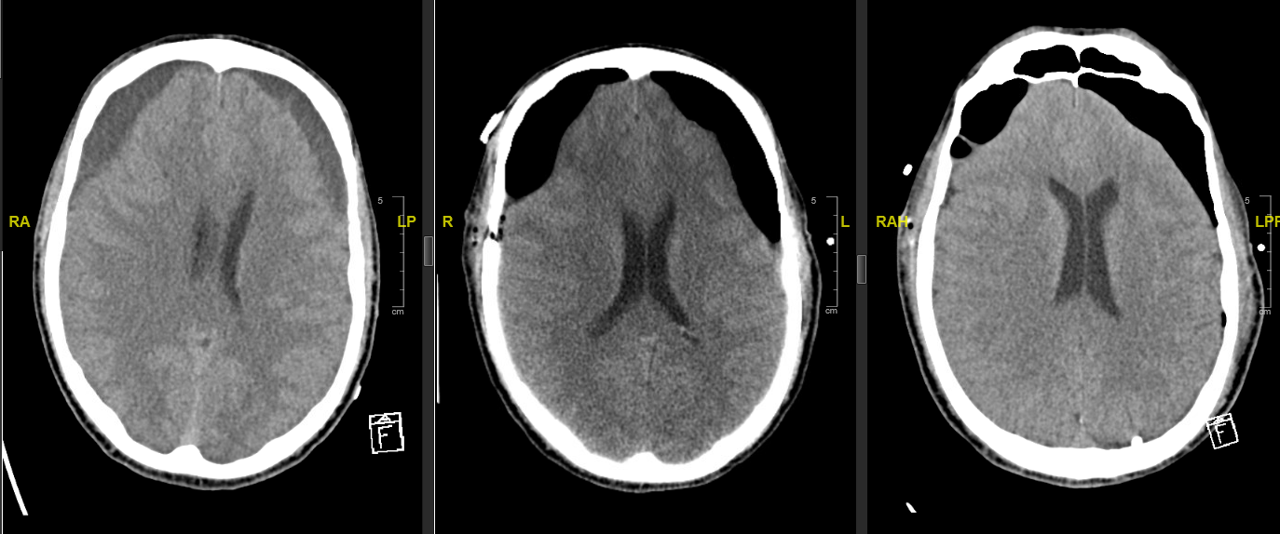
\includegraphics[width=0.8\linewidth]{CTfig2}
\caption{From left to right: Brain CT of 78yoM patient. 
(a) 8/5/21 prior to L mini crani and R burr hole. (b) 8/5/21 9pm postsurgical imaging shows significant pneumocephalus bilaterally. (c) 8/6/21 6am slight improvement of pneumocephalus after conservative treatment and 12 hours of alternating 100\% FiO2 therapy. }
\label{fig:view2}
\end{figure}

\subsection*{Case 1: 83yo with SDH s/p craniotomy}
83 y.o.female PMH Afib/TAVR on lifetime Eliquis/aspirin s/p L craniotomy for evacuation of subdural hematoma after fall from standing with headstrike. Imaging revealed subdural hemorrhage (SDH); Patient had L craniotomy for SDH evacuation. Her physical exam was benign and included a nonfocal neuro exam with no cranial nerve or cognitive deficits. 

Initial CT on arrival (Figure~\ref{fig:view}) revealed a large L frontotemporal holohemispheric EDH and R frontal subacute SDH with no air in frontal area. Post craniotomy, a Mt. Fuji sign can be visualized in the frontal area. 

Patient was treated conservatively without additional oxygen administration due to reassuring exam findings and is currently being monitored for PNC signs. 

\subsection*{Case 2: 78yoM with L mini craniotomy and R burr hole for SDH evacuation}
78yoM PMH hypertension, anemia, bladder cancer s/p left mini craniotomy and R burr hole for SDH evacuation. Patient was found to have bilateral subdural hemorrhage on MRI; initially had epidural blood patch and had weakness, trouble walking and HA. 3 days later, had significant decline in neuro exam. The patient had L craniotomy and R burrhole for b/l subdural hematoma evacuation; postoperative CT showed significant pneumocephalus and patient had continued somnolence (Figure~\ref{fig:view2}.
Patient was treated with alternating 100\% FiO2 for 24 hours. Clinical exam improved significantly after 12 hours of conservative therapy and alternating FiO2 therapy. 


\section*{Acknowledgments}
This report was generated for educational purposes as part of the NCCU rotation at Brown University. Adapted from [1]

\bibliography{sample}

\end{document}